% !TeX spellcheck = cs_CZ
%---------------------------------------------------------------------------------------------------
% file: mai1ch08.tex
%---------------------------------------------------------------------------------------------------
%===================================================================================================
% ------------------------------------------- Definite Integral -----------------------------------
\setchaptertoc
\chapter{Určitý integrál}
  \section{Integrování — „sčítání“ mnoha malých příspěvků} 
    S pojmem integrálu jsme se setkali již v kapitole o derivacích. \emph{Neurčitým integrálem} z
    funkce \(f(x)\) jsme nazývali primitivní funkci \(F(x)\) k zadané funkci \(f(x)\), tj. funkci,
    jejímž derivováním právě \(f(x)\) získáme. Z praktických fyzikálních výpočtů jsme již zvyklí
    počítat \emph{určitý integrál} z funkce \(f(x)\) v mezích \([a, b]\) pomocí takzvané
    \textbf{Leibnizovy-Newtonovy formule} jako 
    \begin{equation}\label{mai:eq100}
      \int_a^bf(x)\dd{x} = [F(x)]_a^b = F(b) - F(a)
    \end{equation}
    Příjemnou vlastností tohoto výsledku je, že dává stejnou hodnotu pro všechny primitivní funkce k
    funkci \(f(x)\). Ty se sice mohou lišit o konstantu, v rozdílu \(F(b) - F(a)\) se však tato
    konstanta nakonec neprojeví, vyruší se. Co však vztah (\ref{mai:eq100}) znamená? A jak je vůbec
    určitý integrál definován? Je vztah (\ref{mai:eq100}) jeho definicí, nebo je důsledkem nějaké
    jiné definice, vybudované třeba na základě geometrických úvah? Pravá podstata integrování je
    skutečně jinde než ve vztahu (\ref{mai:eq100}), i když bezprostřední souvislost s primitivní
    funkcí zde existuje. Myšlenka integrování opravdu vzešla z geometrických požadavků, konkrétně
    požadavku zjišťování délek, obsahů a objemů geometrických útvarů. V současné době existuje celá
    řada typů určitých inte­grálů. Nejnázornější z nich je \textbf{Riemannův integrál}, kterým se
    budeme v tomto odstavci zabývat.

    \begin{figure}[ht!]
      \centering
      \animategraphics[controls,autoplay,loop]{2}{mai_fig022}{}{}
      \caption{text
              (\cite[s.~10000]{Feynman01})}
    \end{figure}

    \begin{figure}[ht!]  %\ref{mai:fig031}
      \centering
      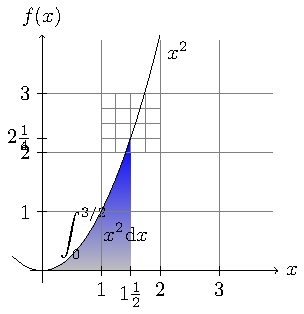
\includegraphics[width=0.7\linewidth]{mai_fig031.pdf}
      \caption{
              (\cite[s.~10000]{Feynman01})}
      \label{mai:fig031}
    \end{figure}

  \subsection{Výpočet integrálu}
      \begin{example}
        Spočítejme integrál $\displaystyle \int_1^{ln5}{(x+1)e^xdx}$  metodou per partes: 
        \begin{align*}
          \int{(x+1)e^xdx} &= \int{e^xdx}+\int{x\cdot e^xdx}     \\
                           &= e^x + (x-1)e^x = xe^x              \\
          \int_1^{ln5}{(x+1)e^xdx} &= [xe^x]_1^{ln5} = 5ln5-e    \\
        \end{align*}
        kde integrál
        \begin{align*}
            \int{xe^xdx}
              &=\left[\begin{array}{cc}
                  u=x   & dv=e^x \\ [-1em]
                  du=dx & v=e^x
                \end{array}\right]= xe^x-\int{e^xdx}  \\
              &= xe^x - e^x+C
        \end{align*}
      \end{example}

\section{Vlastnosti určitého integrálu}
  V této kapitole mluvíme o spojitých funkcích $\Rightarrow$ příslušné integrály tedy vždy
  existují. Čerpáno z knih:
  \cite{Knichal}.

  \begin{lemma}
    \textbf{První věta o střední hodnotě integrálního počtu}: Je-li funkce $f(x)$ spojitá v
    intervalu $\langle a, b\rangle$, existuje alespoň jeden takový bod $c\in(a, b)$, že platí

    \begin{equation}\label{MA:eq_av1}
      \int_a^b f(x)dx = (b-a)f(c).
    \end{equation}
  \end{lemma}

  \begin{proof} Použitím Lagrangeovy věty napsané pro funkci $F(x)$, primitivní na intervalu
    $\langle a, b\rangle$ k dané funkci $f(x)$. Podmínky věty jsou zřejmě splněny: $F(x)$ je
    spojitá na intervalu $\langle a, b\rangle$ a má všude derivaci $F'(x)= f(x)$. Tedy existuje
    alespoň jeden bod $c\in(a, b)$,
    
    \begin{figure}[ht!]  %\ref{mai:fig029}
      \centering
      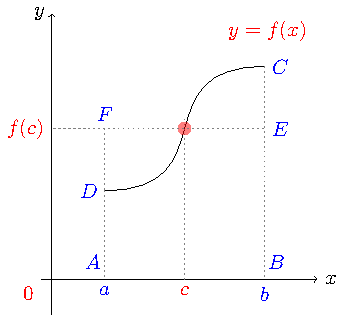
\includegraphics[width=0.7\linewidth]{mai_fig029.pdf}
      \caption{Vztah mezi silou tření a kolmou silou při smýkání
              (\cite[s.~173]{Feynman01})}
      \label{mai:fig029}
    \end{figure}

     že $$F(b)-F(a) = (b-a)F'(c),$$ čímž je věta dokázána, neboť $F(b)-F(a) = \int_a^bf(x)dx$ a
     $F'(c) = f(c)$. Funkční hodnotu $f(c)$, danou podle (\ref{MA:eq_av1}) rovnicí  
     \begin{equation}\label{MA:eq_av2}
        f(c) = \frac{1}{b-a}\int_a^b f(x)dx
     \end{equation}
     nazýváme \texttt{střední hodnotou}.
  \end{proof}

  Pro spojitou nezápornou funkci $f(x)$, lze větu o střední hodnotě jednoduše geometricky
  interpretovat dle (obr.\ref{mai:fig029}). Levá strana (\ref{MA:eq_av1}) určuje obsah
  křivočarého lichoběžníka $ABCD$, pravá strana obsah obdélníka $ABEF$. Podle této věty nabývá
  funkce $f(x)$ aspoň v jednom bodě intervalu $(a, b)$ takové hodnoty $f(c)$, že uvažovaný
  křivočarý lichoběžník má stejný obsah jako obdélník o základně $b-a$ a výšce $f(c)$ (str. 155
  knihy \cite{Knichal}).

  %---------------------------------------------------------------
  % !TeX spellcheck = cs_CZ
\begin{mdframed}[style=mdexam]
  \begin{example}\label{MAI:exam032}
    Určete střední hodnotu $i_s$ střídavého proudu $$i(t) = I_0\sin\omega t$$ v časovém intervalu
    $\langle 0, \frac{T}{2}\rangle$ (v průběhu jedné poloviny periody). $I_0$ je maximální hodnota
    proudu (obr. \ref{MAI:exam032}), perioda $T$ je dána vztahem $T = \frac{2\pi}{\omega}$
    
    {\centering
    \captionsetup{type=figure}
    \luafigure[1]{mai_fig030.pdf}
    \captionof{figure}{K příkladu \ref{MAI:exam032}
    \cite[s.~119]{Brabec1989}
    \label{mai:fig030}}
    \par}

      Podle \ref{MA:eq_av2} bude
      \begin{align*}
      i_s &=  \frac{2}{T}
              \int_0^{\frac{T}{2}}I_0\sin\omega t\dd{t} =
              \frac{2I_0}{T}\left[-\frac{\cos\omega t}{\omega}\right]_0^{\frac{T}{2}}        \\
          &=  \frac{2I_0}{T}\frac{1}{\omega}\left(-\cos\frac{\omega T}{2}+ \cos 0\right)     \\
          &=  \frac{2I_0}{2\pi}(-\cos\pi + \cos 0) = \frac{2}{\pi}I_0 \doteq 0,637 I_0.
    \end{align*}

    Tato hodnota se rovná intenzitě elektrického proudu, při kterém by vodičem v průběhu uvažované
    poloviny periody prošel stejný elektrický náboj jako při proudu střídavém.
  \end{example}
\end{mdframed}
















  %---------------------------------------------------------------

  %---------------------------------------------------------------
  % !TeX spellcheck = cs_CZ
\begin{mdframed}[style=mdexam]
  \begin{example}\label{MAI:exam101}
    Efektivní hodnota $i_{ef}$ střídavého proudu $$i(t) = I_0\sin\omega t$$ (viz
    předchozí příklad) je definována jako odmocnina ze střední hodnoty funkce $i^2(t)$ v průběhu
    jedné periody $T = \frac{2\pi}{\omega}$. Tedy
    \begin{align*}
      i_{ef}^2 &= \frac{1}{T}\int_0^T I_0^2\sin^2\omega t\dd{t} = 
                  \frac{1}{T}\int_0^T \frac{I_0^2}{2}(1- \cos2\omega t)\dd{t}           \\
               &= \frac{I_0^2}{2T}
                  \left[
                    t-\frac{\sin2\omega t}{2\omega}
                  \right]_0^T = \frac{I_0^2}{2}
    \end{align*}
    neboť $\sin2\omega T=\sin4\pi = 0.$ Odtud $$i_{ef} = \frac{I_0}{\sqrt{2}}.$$ Střídavý proud
    $i(t) = I_0\sin\omega t$ má na témže odporu stejný výkon jako stejnosměrný proud o intenzitě
    $i = 0,707I_0$.
  \end{example}
\end{mdframed}
















  %---------------------------------------------------------------

  Následující věta může být využita k odhadu některých integrálů
  \begin{lemma}
    \textbf{Druhá věta o střední hodnotě integrálního počtu}: Jsou-li funkce $f(x)$ a $g(x)$
    spojité v intervalu $\langle a, b \rangle$ a je-li funkce $g(x)$ v $\langle a, b \rangle$
    nezáporná a nerostoucí, existuje alespoň jeden bod $c\in\langle a, b \rangle$ tak, že platí
    \begin{equation}\label{MA_eq_av3}
        \int_a^b f(x)g(x) = g(a)\int_a^c f(x)dx.
    \end{equation}
  \end{lemma}
  Zcela obdobnou větu lze vyslovit pro případ, že $g(x)$ je v intervalu $\langle a, b \rangle$
  nezáporná a neklesající, tj. na pravé straně \ref{MA_eq_av3} je pak integrál $g(b)\int_c^b
  f(x)dx$

   %--Odhad hodnoty integrálu \int_{100\pi}^{1000\pi}\frac{\sin x}{x}dx---------
   % !TeX spellcheck = cs_CZ
\begin{mdframed}[style=mdexam]
  \begin{example}\label{mai:exam097}
    Odhadněte hodnotu integrálu:
    \begin{equation}\label{MA_eq_sinx_x}
        \int_{100\pi}^{1000\pi}\frac{\sin x}{x}dx
    \end{equation}
    Řešení: Funkce $f(x) = \sin x$ a $g(x) = \frac{1}{x}$ jsou v uvažovaném intervalu $\langle
    100\pi, 1000\pi \rangle$ spojité a funkce $g(x)$ je kladná a nerostoucí.
    \begin{align*}
      \int_{100\pi}^{1000\pi}\frac{\sin x}{x}dx 
        &=\frac{1}{100\pi}\int_{100\pi}^c\sin xdx                                   \\
        &=\frac{1}{100\pi}\left(\cos100\pi - \cos c\right)
    \end{align*}
    kde $c$ je kladné číslo z intervalu $\langle 100\pi, 1000\pi \rangle$. Dále pro všechna
    $c\in\langle 100\pi, 1000\pi \rangle$ platí $0\leq1-\cos c\leq2$, takže
    \begin{equation*}
        0\leq\int_{100\pi}^{1000\pi}\frac{\sin x}{x}dx\leq \frac{1}{50\pi}.
    \end{equation*}
  \end{example}  
\end{mdframed}
   %----------------------------------------------------------------------------

\section{Numerický výpočet integrálu pomocí Matlabu}
  Matlab obsahuje dvě funkce pro výpočet určitého integrálu |quad| a |quadl|. Výpočet je založen na
  \emph{numerické kvadratuře}. Funkce |quad| využívá pro výpočet rekurzivní adaptivní Simpsonovo
  pravidlo. Příkaz |quad(fce,a,b)| vypočte určitý integrál funkce \emph{fce}, kde \emph{fce} je
  odkaz na funkci, \(a\) a \(b\) jsou meze integrace. Meze integrace musí být konečné. 

  Použití si ukážeme na příkladu výpočtu určitého inegrálu následující funkce
  \begin{equation*}
    \int_0^\pi x\cdot\sin{x}\dd{x}
  \end{equation*}
  Nejprve je potřeba nadefinovat funkci, kterou chceme integrovat (\(y=x\cdot\sin{x}\)), pomocí
  funkce Matlabu. Nazveme tuto funkci |int\_xsinus| a uložíme ji do zvláštního souboru 
  \begin{lstlisting}[style=luaMatlabStyle] 
        function [y] = int_xsinus(x)
        y = x.*sin(x);
  \end{lstlisting} 
  Výpočet integrálu pak provedeme pomocí funkce |quad(@int\_xsinus, 0, pi)|, kde první parametr je
  odkaz na funkci |int\_xsinus| a druhé dva parametry jsou meze integrace.
  \begin{lstlisting}[style=luaMatlabStyle] 
        >> quad(@int_xsinus, 0 , pi)
        ans = 3.1416
  \end{lstlisting}  
  Funkci je možné také definovat jako anonymní funkci, zápis se zkrátí a zpřehlední
  \begin{lstlisting}[style=luaMatlabStyle]  
        >> xsinus = @(x) x.*sin(x); % anonymni funkce
        >> quad(xsinus, 0, pi)      % vypocet integralu
        ans = 3.1416
  \end{lstlisting}
  Hodnota určitého integrálu na intervalu od \(0\) do \(\pi\) bude tedy \(\int_0^\pi
  x\cdot\sin{x}\dd{x} =\num{3.1416}\)

  Následující kód vypočítá hodnotu určitého integrálu zadané funkce a vykreslí graf integrované
  funkce a jejího integrálu.

  \lstinputlisting[style=luaMatlabStyle, caption=\texttt{int\_xsinus\_graph.m}: Výpis programu  
          druhého.]{../src/MAI/matlab/int_xsinus_graph.m}

  Určitý integrál je možné interpretovat jako plochu pod modrou křivkou na obrázku xx. Červená
  křivka zobrazuje hodnotu určitého integrálu v mezích od nuly do \(\pi\).

  Funkce |quadl| používá \emph{rekurzivní adaptivní Lobattovo kvadratur}. Tento postup je možné
  použí pro výpočet integrálu s větší přesností, nebo pokud integrace s |quad| selže. 

  Standardně je nastavena tolerance pro absolutní chybu menší než \num{e-6}. Tuto toleranci je možné
  změnit dalším parametrem funkcí ro integraci |quad(fce, a, b, tol)|.

%} %tikzset
%---------------------------------------------------------------------------------------------------